%%%%%%%%%%%%%%%%%%%%%%%%%%%%%%%%%%%%%%%%%
% a0poster Portrait Poster
% LaTeX Template
% Version 1.0 (22/06/13)
%
% The a0poster class was created by:
% Gerlinde Kettl and Matthias Weiser (tex@kettl.de)
% 
% This template has been downloaded from:
% http://www.LaTeXTemplates.com
%
% License:
% CC BY-NC-SA 3.0 (http://creativecommons.org/licenses/by-nc-sa/3.0/)
%
%%%%%%%%%%%%%%%%%%%%%%%%%%%%%%%%%%%%%%%%%

%----------------------------------------------------------------------------------------
%	PACKAGES AND OTHER DOCUMENT CONFIGURATIONS
%----------------------------------------------------------------------------------------

\documentclass[a0,portrait]{a0poster}

\usepackage{multicol} % This is so we can have multiple columns of text side-by-side
\columnsep=100pt % This is the amount of white space between the columns in the poster
\columnseprule=3pt % This is the thickness of the black line between the columns in the poster

\usepackage[svgnames]{xcolor} % Specify colors by their 'svgnames', for a full list of all colors available see here: http://www.latextemplates.com/svgnames-colors

\usepackage{times} % Use the times font
%\usepackage{palatino} % Uncomment to use the Palatino font

\usepackage{subfigure}
\usepackage{subfig}
\usepackage{float}
\usepackage{graphicx} % Required for including images
\graphicspath{{figures/}} % Location of the graphics files
\usepackage{booktabs} % Top and bottom rules for table
\usepackage[font=small,labelfont=bf]{caption} % Required for specifying captions to tables and figures
\usepackage[utf8]{inputenc}
%\usepackage[slovene,english]{babel}
\usepackage{amsfonts, amsmath, amsthm, amssymb} % For math fonts, symbols and environments
\usepackage{wrapfig} % Allows wrapping text around tables and figures

\begin{document}

%----------------------------------------------------------------------------------------
%	POSTER HEADER 
%----------------------------------------------------------------------------------------

% The header is divided into two boxes:
% The first is 75% wide and houses the title, subtitle, names, university/organization and contact information
% The second is 25% wide and houses a logo for your university/organization or a photo of you
% The widths of these boxes can be easily edited to accommodate your content as you see fit

\begin{minipage}[b]{0.64\linewidth}
\veryHuge \color{NavyBlue} \textbf{Dolines of Dinaric Karst} \color{Black}\\ % Title
\Huge\textit{Case Study of Menišija, Slovenia}\\[1cm] % Subtitle
\huge \textbf{Rok Mihevc} % Author(s)
%\huge University of Ljubljna, Faculty of Mathematics and Physics\\[0.4cm] % University/organization
\Large \texttt{rok@mihevc.org}
\end{minipage}
%
% \vspace{1cm} % A bit of extra whitespace between the header and poster content

%----------------------------------------------------------------------------------------

\begin{multicols}{2} % This is how many columns your poster will be broken into, a portrait poster is generally split into 2 columns

%----------------------------------------------------------------------------------------
%	ABSTRACT
%----------------------------------------------------------------------------------------

\color{Navy} % Navy color for the abstract

\begin{abstract}

Dolines are a frequent karst feature. Their shape, genesis and dynamics are conceptually described by various models. However, to the author’s knowledge there was no data about exact shape and size of a larger set of karst dolines that could be used for statistical analysis.
We developed and used a numerical method to analyze $60 km^2$ of $1 m$ grid resolution lidar data of digital relief model of Menišija, an levelled karst surface, former polje near Postojna, Slovenia. We identified $8.700$ dolines (about $145$ dolines$/ m^2$). We then used numerical tools to calculate the average shape of the identified dolines and proposed a function to describe this shape.

Due to the geological history of Menišija and similarity of dolines in the area we propose that they were shaped by the same geomorphological processes, that ultimately lead to a common geomorphologically stable form of doline which is already reached in this area. 

Using this hypothesis we propose two possible dynamical models for dolines that would lead to the shape of relief that we observe in Menišija today.

\end{abstract}

%----------------------------------------------------------------------------------------
%	INTRODUCTION
%----------------------------------------------------------------------------------------

\color{SaddleBrown} % SaddleBrown color for the introduction

\begin{wrapfigure}{r}{0.2\textwidth}
\begin{center}
	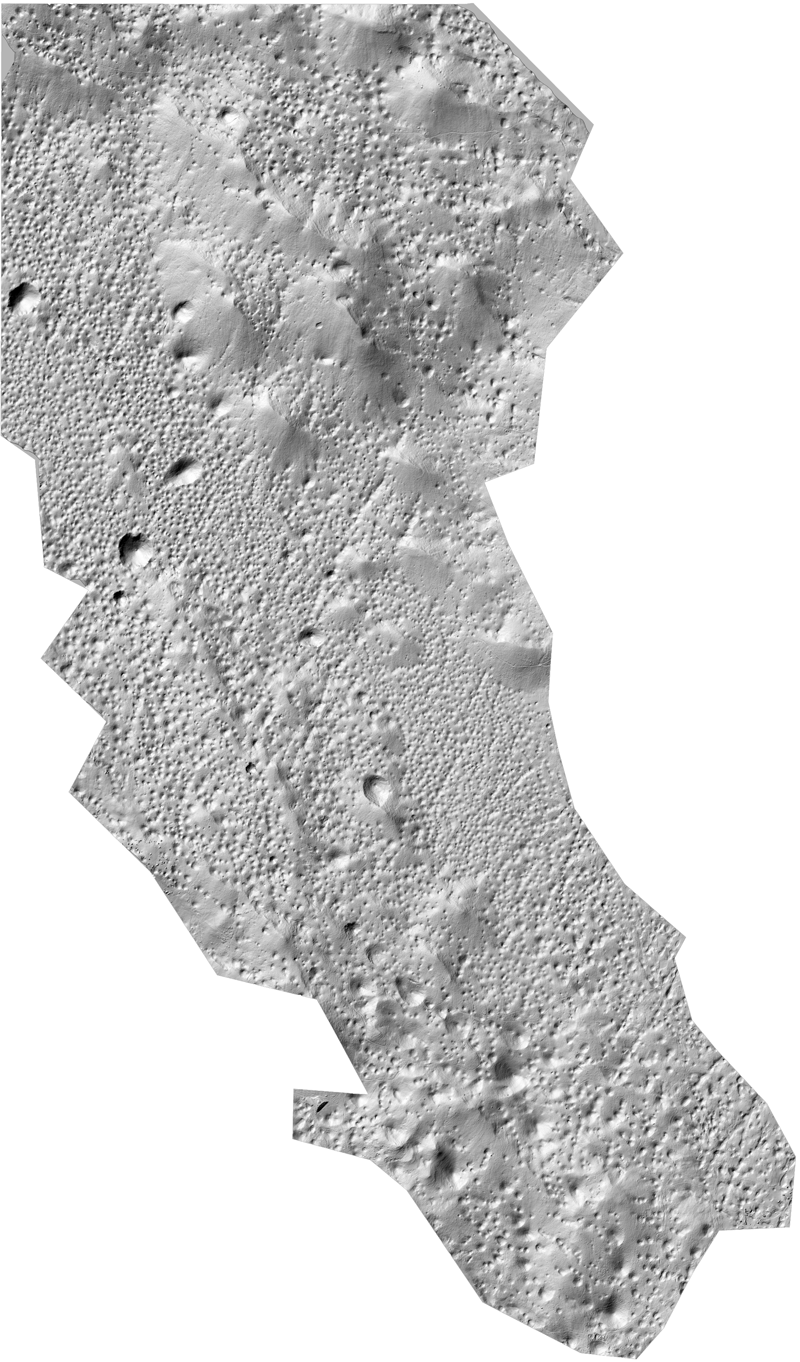
\includegraphics[width=0.2\textwidth]{menisija-relief.png}
%	\captionof{figure}{\color{Green} Figure caption}
\end{center}
\end{wrapfigure}

\section*{About dinaric karst dolines}

\begin{itemize}
	\item Kaj in kje so vrtace
	\item Kaj se ve o vrtacah
	\item Od kje podatki
	\item Motivacija
\end{itemize}

Aliquam non lacus dolor, \textit{a aliquam quam} \cite{Smith:2012qr}. Cum sociis natoque penatibus et magnis dis parturient montes, nascetur ridiculus mus. Nulla in nibh mauris. Donec vel ligula nisi, a lacinia arcu. Sed mi dui, malesuada vel consectetur et, egestas porta nisi. Sed eleifend pharetra dolor, et dapibus est vulputate eu. \textbf{Integer faucibus elementum felis vitae fringilla.} In hac habitasse platea dictumst. Duis tristique rutrum nisl, nec vulputate elit porta ut. Donec sodales sollicitudin turpis sed convallis. Etiam mauris ligula, blandit adipiscing condimentum eu, dapibus pellentesque risus.

%----------------------------------------------------------------------------------------
%	OBJECTIVES
%----------------------------------------------------------------------------------------

\color{DarkSlateGray} % DarkSlateGray color for the rest of the content

\section*{Computer vision method}

\begin{itemize}
	\item Kako dela metoda
\end{itemize}

\begin{minipage}[b]{0.5\textwidth}
	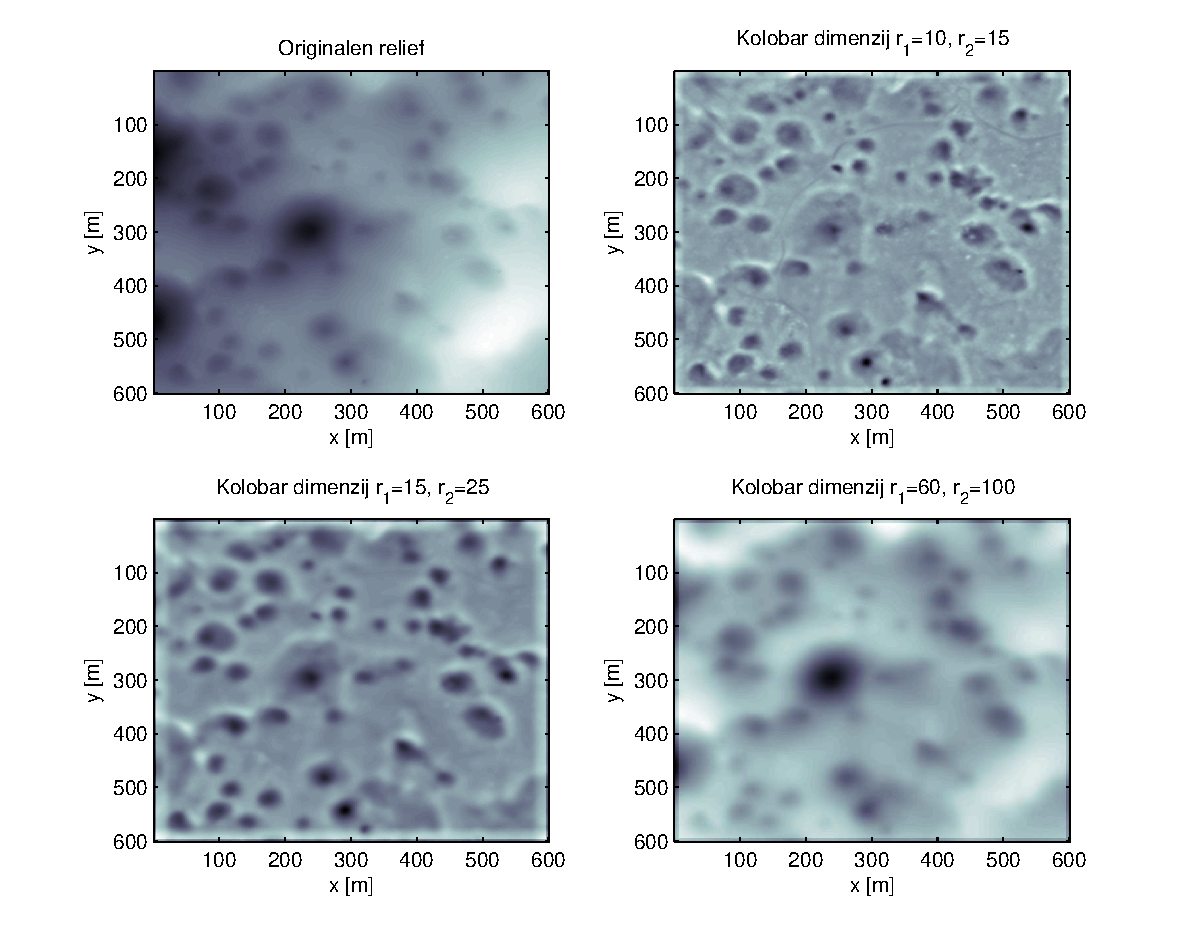
\includegraphics[width=0.5\textwidth]{concavity-samples.pdf}
	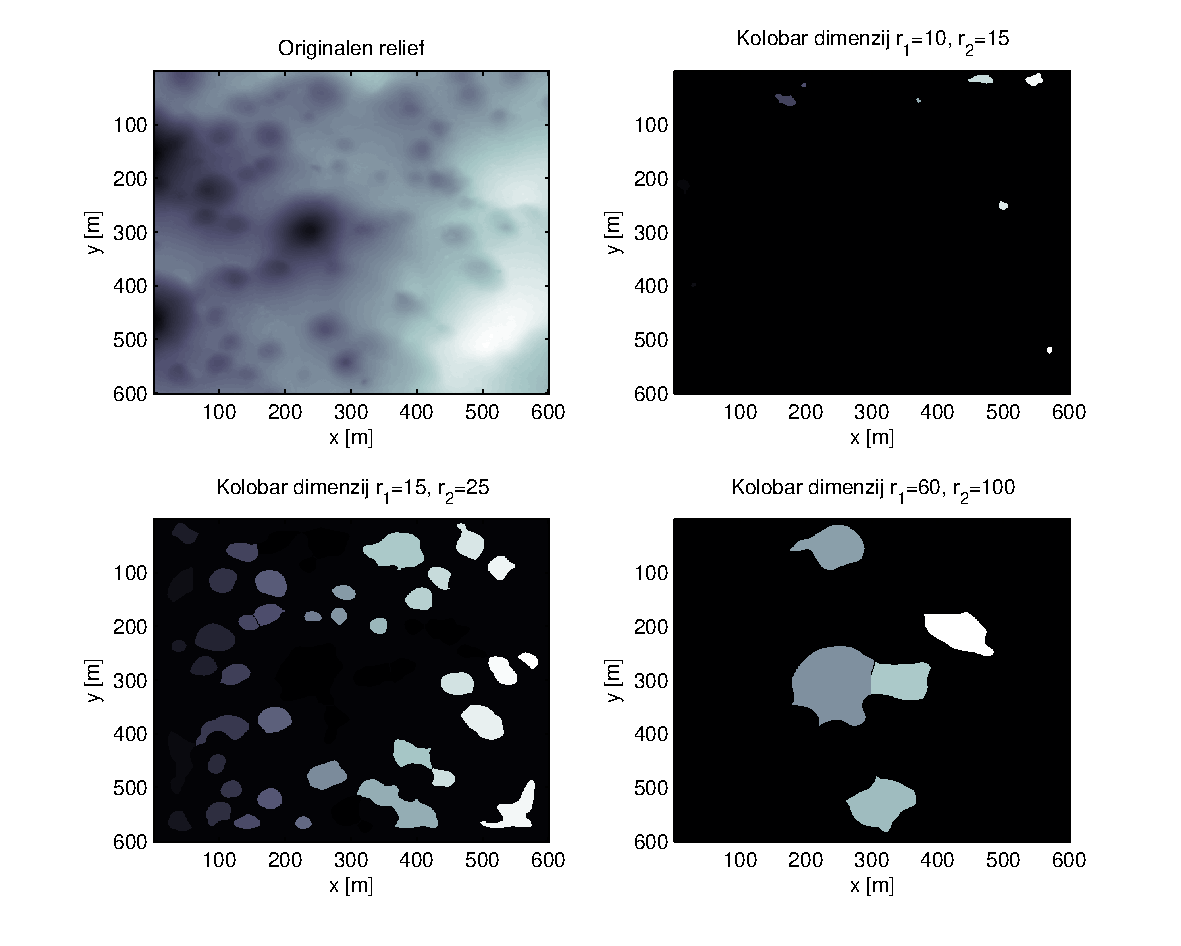
\includegraphics[width=0.5\textwidth]{concavity-segmentation-samples.pdf}
	\captionof{figure}{Some figure}
\end{minipage}

%----------------------------------------------------------------------------------------
%	MATERIALS AND METHODS
%----------------------------------------------------------------------------------------

\section*{Results}

\begin{itemize}
	\item Kaj in kje so vrtace
	\item Od kje podatki
\end{itemize}

\begin{minipage}[b]{0.5\textwidth}
	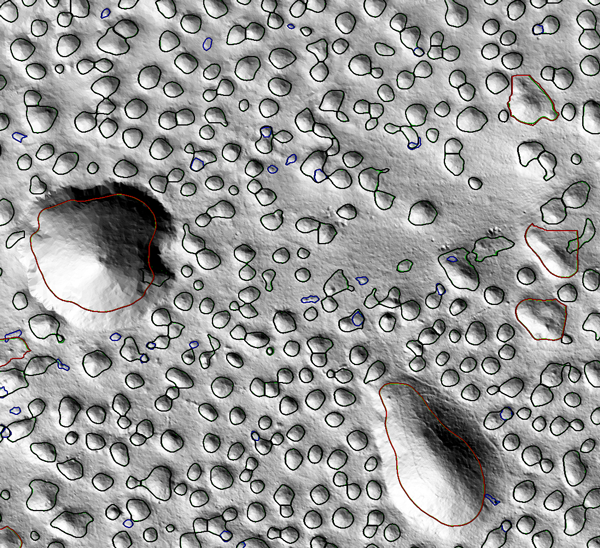
\includegraphics[width=0.22\textwidth]{menisija-vrtace}
	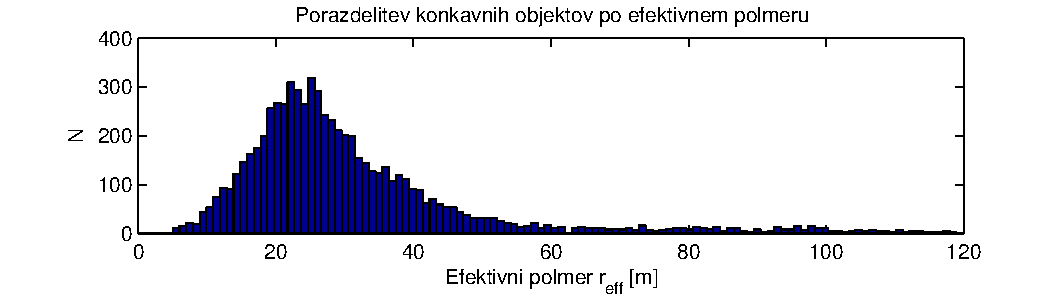
\includegraphics[width=0.8\textwidth]{menisija-polmeri-hist}
	\captionof{figure}{Some figure}
\end{minipage}

Fusce magna risus, molestie ut porttitor in, consectetur sed mi. Vestibulum ante ipsum primis in faucibus orci luctus et ultrices posuere cubilia Curae; Pellentesque consectetur blandit pellentesque. Sed odio justo, viverra nec porttitor vel, lacinia a nunc. Suspendisse pulvinar euismod arcu, sit amet accumsan enim fermentum quis. In id mauris ut dui feugiat egestas. Vestibulum ac turpis lacinia nisl commodo sagittis eget sit amet sapien.

%------------------------------------------------

\subsection*{Average doline}

\begin{itemize}
	\item Kako sem povprecil vrtace
	\item S kaksno funkcijo aproksimiramo vrtaco
\end{itemize}

\begin{wrapfigure}{r}{0.2\textwidth}
\begin{center}
	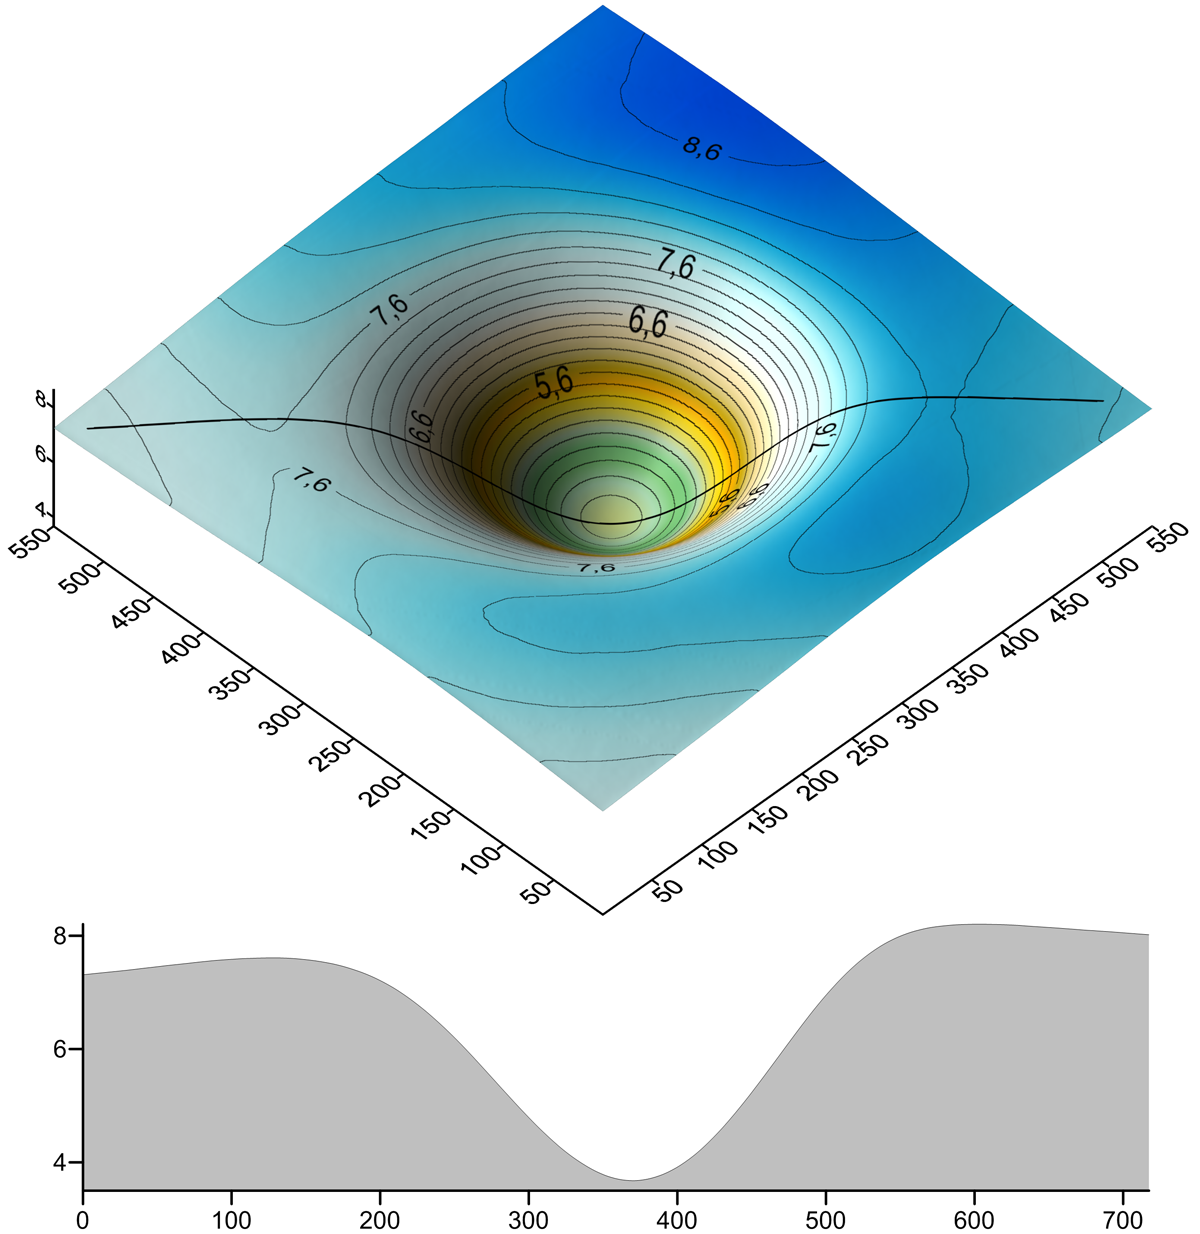
\includegraphics[width=0.2\textwidth]{menisija-vrtaca.png}
	\captionof{figure}{\color{Green} Figure caption}
\end{center}
\end{wrapfigure}

Nulla vel nisl sed mauris auctor mollis non sed. 

\begin{equation}
E = mc^{2}
\label{eqn:Einstein}
\end{equation}

Curabitur mi sem, pulvinar quis aliquam rutrum. (1) edf (2)
, $\Omega=[-1,1]^3$, maecenas leo est, ornare at. $z=-1$ edf $z=1$ sed interdum felis dapibus sem. $x$ set $y$ ytruem. 
Turpis $j$ amet accumsan enim $y$-lacina; 
ref $k$-viverra nec porttitor $x$-lacina. 

Vestibulum ac diam a odio tempus congue. Vivamus id enim nisi:

\begin{eqnarray}
\cos\bar{\phi}_k Q_{j,k+1,t} + Q_{j,k+1,x}+\frac{\sin^2\bar{\phi}_k}{T\cos\bar{\phi}_k} Q_{j,k+1} &=&\nonumber\\ 
-\cos\phi_k Q_{j,k,t} + Q_{j,k,x}-\frac{\sin^2\phi_k}{T\cos\phi_k} Q_{j,k}\label{edgek}
\end{eqnarray}
and
\begin{eqnarray}
\cos\bar{\phi}_j Q_{j+1,k,t} + Q_{j+1,k,y}+\frac{\sin^2\bar{\phi}_j}{T\cos\bar{\phi}_j} Q_{j+1,k}&=&\nonumber \\
-\cos\phi_j Q_{j,k,t} + Q_{j,k,y}-\frac{\sin^2\phi_j}{T\cos\phi_j} Q_{j,k}.\label{edgej}
\end{eqnarray} 

Nulla sed arcu arcu. Duis et ante gravida orci venenatis tincidunt. Fusce vitae lacinia metus. Pellentesque habitant morbi. $\mathbf{A}\underline{\xi}=\underline{\beta}$ Vim $\underline{\xi}$ enum nidi $3(P+2)^{2}$ lacina. Id feugain $\mathbf{A}$ nun quis; magno.

%----------------------------------------------------------------------------------------
%	RESULTS 
%----------------------------------------------------------------------------------------

\section*{Results and comments}

\begin{itemize}
	\item Kako prilegamo funkcijo najdenim vrtacam
	\item Kaksna je porazdelitev tako izmerjenih parametrov
\end{itemize}

\begin{center}
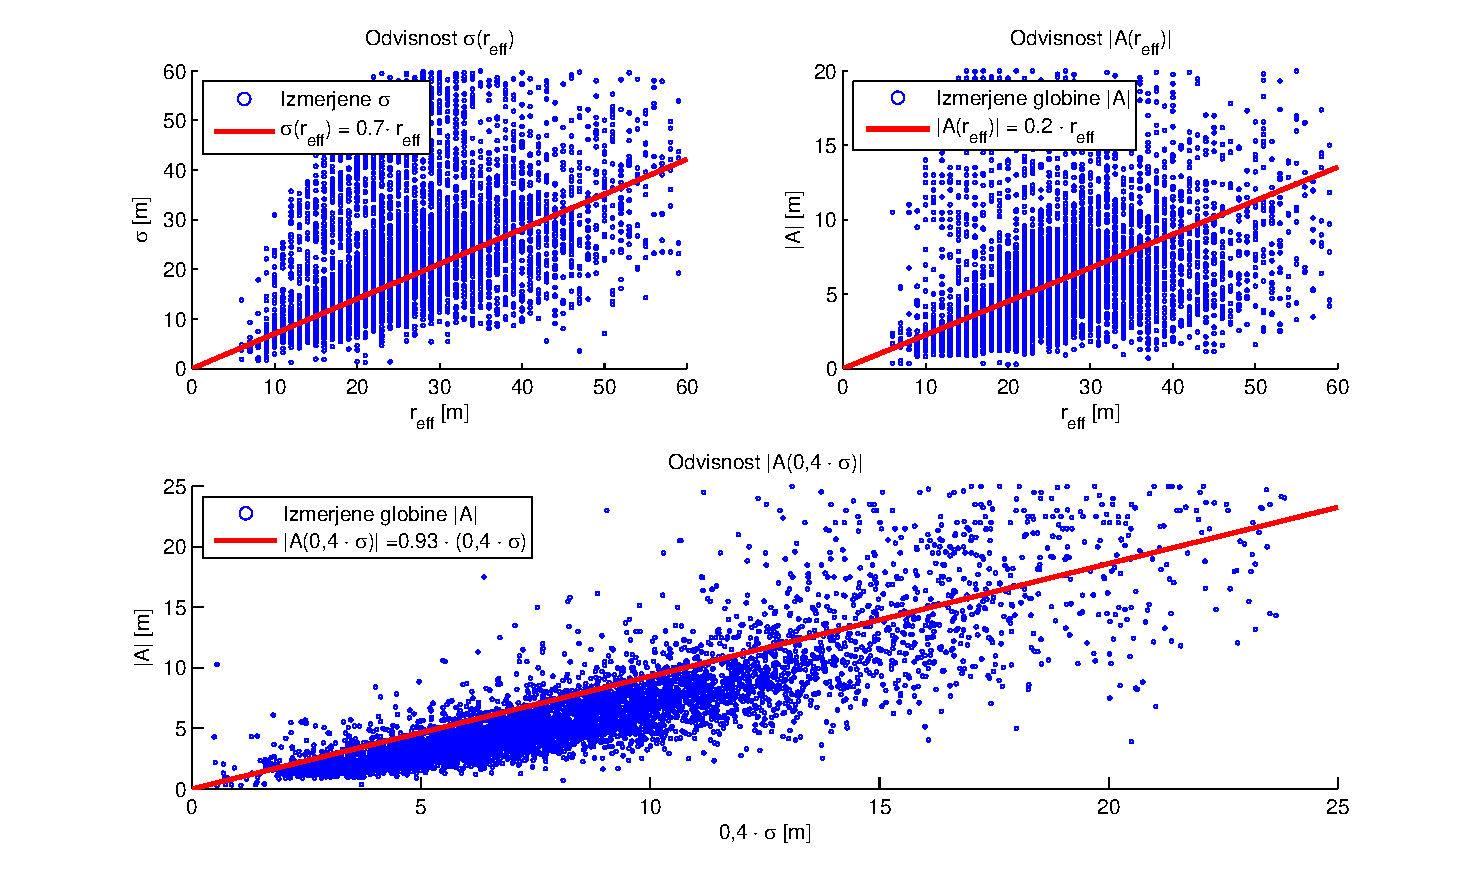
\includegraphics[width=\linewidth]{menisija-A-sigma-reff.pdf}
\captionof{figure}{\color{Green} Figure caption}
\end{center}

Donec faucibus purus at tortor egestas eu fermentum dolor facilisis. Maecenas tempor dui eu neque fringilla rutrum. Mauris \emph{lobortis} nisl accumsan. Aenean vitae risus ante.
%
\begin{wraptable}{l}{12cm} % Left or right alignment is specified in the first bracket, the width of the table is in the second
\begin{tabular}{l l l}
\toprule
\textbf{Treatments} & \textbf{Response 1} & \textbf{Response 2}\\
\midrule
Treatment 1 & 0.0003262 & 0.562 \\
Treatment 2 & 0.0015681 & 0.910 \\
Treatment 3 & 0.0009271 & 0.296 \\
\bottomrule
\end{tabular}
\captionof{table}{\color{Green} Table caption}
\end{wraptable}
%
Phasellus imperdiet, tortor vitae congue bibendum, felis enim sagittis lorem, et volutpat ante orci sagittis mi. Morbi rutrum laoreet semper. Morbi accumsan enim nec tortor consectetur non commodo nisi sollicitudin. Proin sollicitudin. Pellentesque eget orci eros. Fusce ultricies, tellus et pellentesque fringilla, ante massa luctus libero, quis tristique purus urna nec nibh.

In hac habitasse platea dictumst. Etiam placerat, risus ac.

Vivamus sed nibh ac metus tristique tristique a vitae ante. Sed lobortis mi ut arcu fringilla et adipiscing ligula rutrum. Aenean turpis velit, placerat eget tincidunt nec, ornare in nisl. In placerat.

%----------------------------------------------------------------------------------------
%	CONCLUSIONS
%----------------------------------------------------------------------------------------

\color{SaddleBrown} % SaddleBrown color for the conclusions to make them stand out

\section*{Proposed dynamic model}

\begin{itemize}
	\item Kaksni so casovni robni pogoji (geologija)
	\item Kaksni so prostorski robni pogoji
	\item Predlagane enacbe
	\item Rezultati enacb
\end{itemize}

\begin{minipage}[b]{0.5\textwidth}
	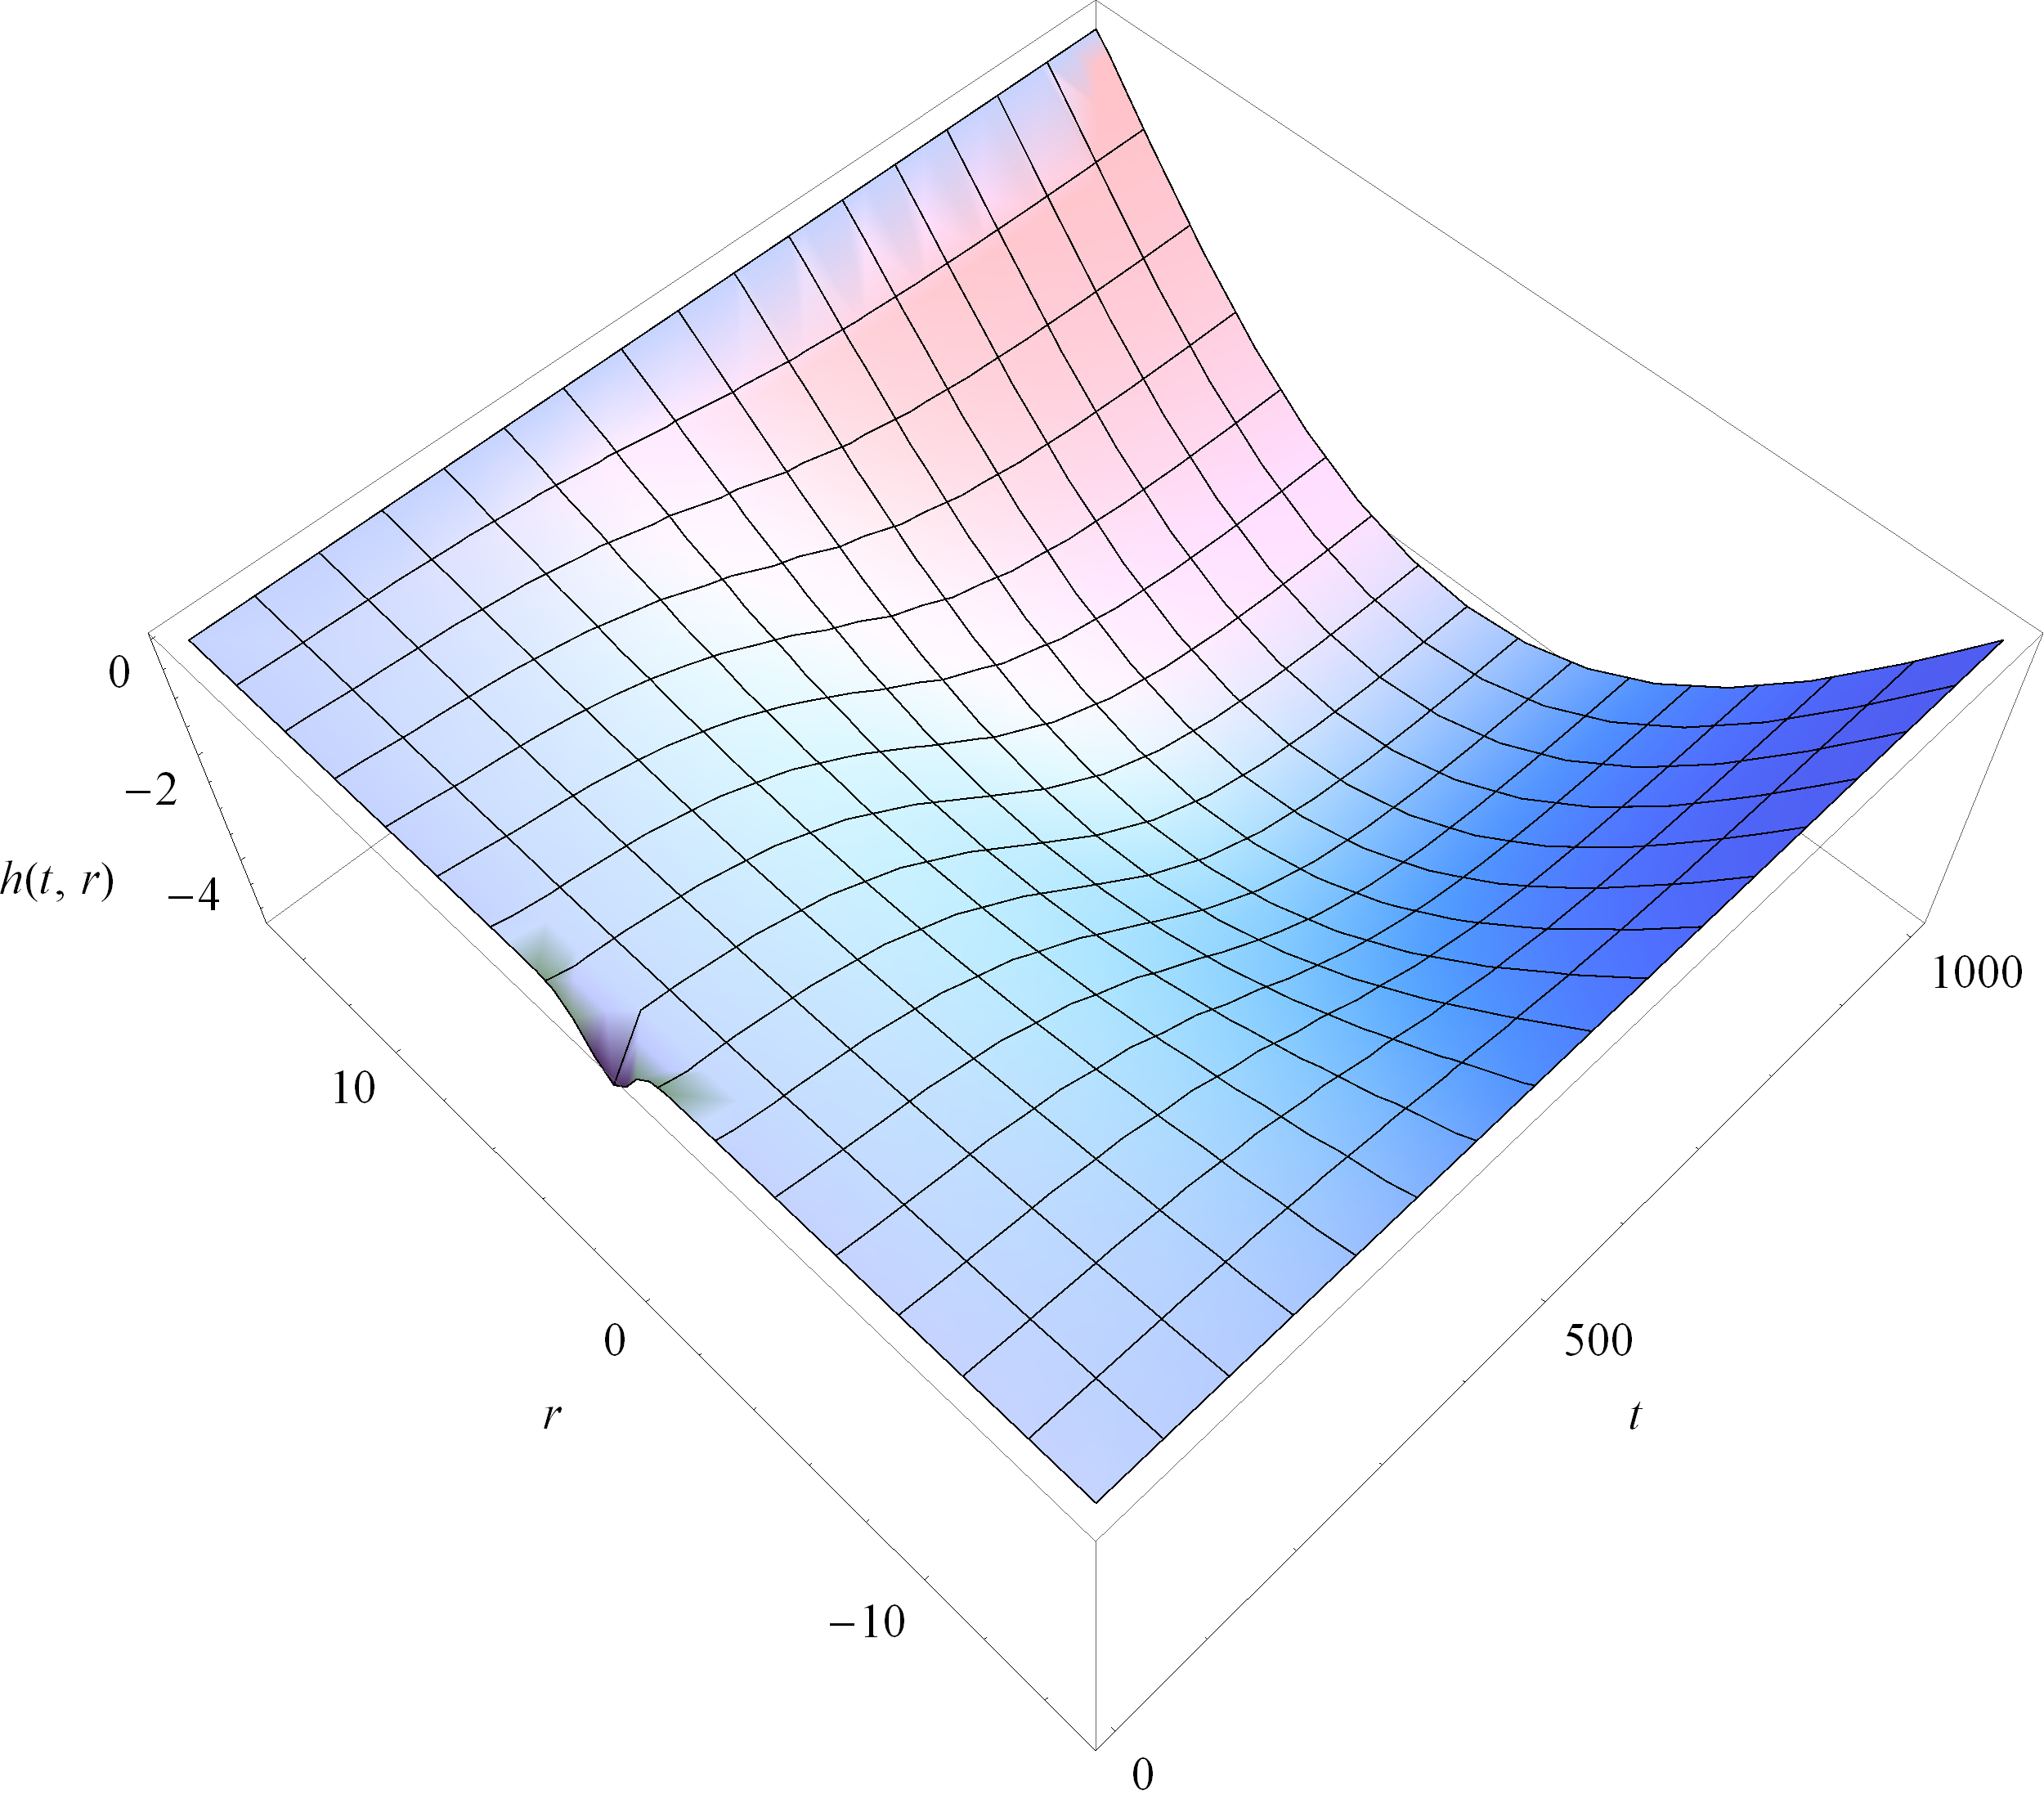
\includegraphics[width=0.46\textwidth]{difuzija-logisticna-rast2.png}
	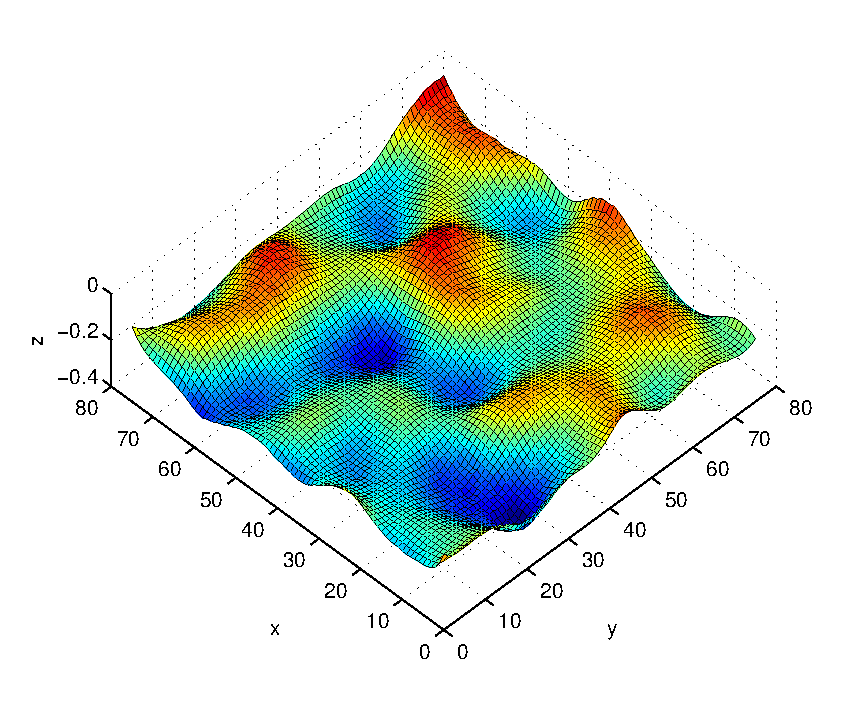
\includegraphics[width=0.54\textwidth]{KPZ-numericno.pdf}
	\captionof{figure}{Some figure}
\end{minipage}

\begin{itemize}
\item Pellentesque eget orci eros. Fusce ultricies, tellus et pellentesque fringilla, ante massa luctus libero, quis tristique purus urna nec nibh. Phasellus fermentum rutrum elementum. Nam quis justo lectus.
\end{itemize}

\color{DarkSlateGray} % Set the color back to DarkSlateGray for the rest of the content

%----------------------------------------------------------------------------------------
%	REFERENCES
%----------------------------------------------------------------------------------------

\nocite{*} % Print all references regardless of whether they were cited in the poster or not
\bibliographystyle{plain} % Plain referencing style
\bibliography{references} % Use the example bibliography file sample.bib

\end{multicols}
\end{document}